\section{Introduktion} % Claes
\subsection{Vesikler og meningen med detektionen - Cryo-EM} % Claes
En celle i nervesystemet kaldes for en neuron eller en nervecelle. En neuron er den vigtigste del i nervesystemet, der bl.a. indeholder hjernen og rygsøjlen. Nerveceller har bl.a. til opgave at modtage og sende information ved hjælp af elektriske og kemiske signaler. I en nervecelle er der så en række synaptiske vesikler, der indeholder neurotransmitters. Når en nervecelle skal sende et impulssignal til en anden nervecelle, bevæger den synaptiske vesikel sig til kanten af nervecellen og udsender neurotransmitters. Nervecellerne genskaber så de synaptiske vesikler så der igen kan sendes nye signaler. To nerveceller hvor der er markeret en synaptisk vesikel i den øverste ses i \ref{fig:syntrans}. I den menneskelige hjerne har en synaptisk vesikel en gennemsnitlig diameter på 39.5 nanometer med en standard afvigelse på 5.1 nanometer.

\begin{figure}[H]
	\centering
	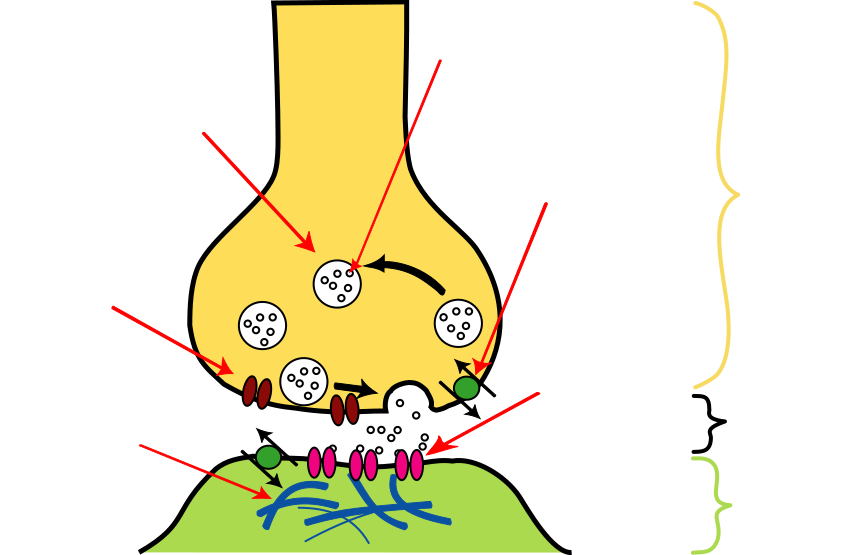
\includegraphics[scale=0.3]{files/intro/img/synTransmitter.png}
	\caption{To neuroner, en afsender af neurotransmitters (A) og en modtager (B). Pilen peger på en synaptisk vesikel.\label{fig:syntrans}}
\end{figure} 

Ved at se på vesiklers placering i forhold til hinanden i celler, kan man afgøre om personen er deprimeret eller ej. Igangværende forskning går i øjeblikket ud på at finde ud af hvorvidt depression er arvelig fra mor til barn, hvis moderen er deprimeret under graviditeten. Vores problem går ud på at lave et system der kan hjælpe forskerne med at detektere disse vesikler i en celle. Det videre arbejde med projektet er så at bruge denne detektion af vesikler til at analysere deres placering i forhold til hinanden, og altså automatisere hele proceduren. Vores problem går bare ud på at detektere.

\subsection{Ground truth}									% Claes
\subsection{Hvad ønsker vi at finde- Målsætning}			% Claes

%% Kildehenvisninger
% http://en.wikipedia.org/wiki/Synaptic_vesicle
% http://en.wikipedia.org/wiki/Neurotransmitter
% http://en.wikipedia.org/wiki/Neuron
% http://en.wikipedia.org/wiki/Cryogenic
% http://en.wikipedia.org/wiki/Cryo-electron_microscopy
